长程智能体的广泛采用使模型工作负载日益呈现出输入密集（input-heavy）的特征。尽管已有
工作大幅降低了长上下文计算的开销，预填充（prefill）阶段的计算成本仍然高昂，且庞大的
KV 缓存持续给 HBM 与 SSD 容量以及数据传输带宽带来压力。计算、存储与带宽三方面的
需求共同构成了进一步降低部署成本的主要瓶颈。为应对这一挑战，我们提出了
DeepSeek-V4.1-Flash：一个多模态混合专家（Mixture-of-Experts，MoE）模型，主干参数
规模为 552B，支持最长一百万 token 的上下文。凭借其因果编码器-解码器
（Causal Encoder-Decoder，CED）架构，模型在解码阶段每 token 激活 16B 参数，
在预填充阶段则仅激活 8B 参数，显著提升了智能体工作负载的成本效率。为突破 KV
缓存压缩的极限，DeepSeek-V4.1-Flash 在压缩稀疏注意力 2（Compressed Sparse
Attention 2，CSA2）中结合了跨层 KV 缓存复用，并采用 FP4 KV 缓存。这些设计将其
全局 KV 缓存占用（始终驻留于 HBM）降至每 token 890 字节，约为 DeepSeek-V4-
Flash 相应占用的 1/4。此外，通过一项名为 SWA Bounded Replay 的专用部署优化，
DeepSeek-V4.1-Flash 将其持久化 KV 缓存占用（始终驻留于 SSD 或主机内存）降至
DeepSeek-V4-Flash 的约 1/8。尽管 KV 缓存占用大幅减小，该模型仍取得了比基线明显
更优的性能。此外，我们对 DeepSeek-V4 的架构进行了精简，并引入了多项高效的架构
扩展。我们在包含 45T token 的多模态语料上对 DeepSeek-V4.1-Flash 进行预训练，并
开展全面的后训练，在多种纯文本与多模态智能体场景中均取得了强劲的性能。模型检查点
可在 https://huggingface.co/deepseek-ai/DeepSeek-V4.1-Flash 获取。

\subsection{1. 引言}\label{introduction}

近年来，长程智能体的应用迅速扩展，使超长上下文处理成为日益重要的模型工作负载。
支持此类工作负载不仅需要高效的长序列处理，还需要对大型 KV 缓存进行持久化存储、
复用与迁移。因此，KV 缓存管理已成为模型部署的一项基础能力，同时也给计算、存储与
通信带来了巨大挑战。此前在稀疏注意力方面的进展 (DeepSeek-AI, 2025, 2026b) 显著
降低了长序列处理的计算成本，使持久化存储与数据搬运日益成为突出的瓶颈。

具体而言，DeepSeek-V4 (DeepSeek-AI, 2026b) 将覆盖整个上下文的全局注意力分支与
局部滑动窗口注意力（Sliding-Window Attention，SWA）相结合。全局分支维护全局 KV，
包括主 KV 与索引器 K，而 SWA 维护局部 KV 状态。在窗口大小固定的情况下，SWA 的
KV 存储量有界，与序列长度无关。因此，对于足够长的序列，全局 KV 主导了运行时 KV
占用，而后者受限于 HBM 容量。此外，部分 KV 会被持久化以用于前缀复用，称之为持久化
KV 缓存，其受限于 SSD 与主机内存容量。I/O 与互连带宽同样限制了缓存的迁移与加载。
这些约束共同限制了服务吞吐，推高了部署成本，并最终阻碍了智能体在更长任务周期与
更广泛应用场景中的部署与采用。

因此，进一步减小 KV 缓存占用对于缓解存储与通信瓶颈、降低长上下文服务成本至关重要。
为此，我们开发了 DeepSeek-V4.1-Flash：一个面向更激进 KV 缓存压缩而设计的多模态
混合专家（MoE）模型。DeepSeek-V4.1-Flash 拥有 552B 主干参数，原生支持多模态输入，
可容纳最长一百万 token 的上下文。我们采用因果编码器-解码器（CED）架构，解码器全局
KV 由编码器最终隐藏状态投影得到。该设计使模型在预填充阶段每 token 激活 8B 参数，
解码阶段激活 16B 参数，对输入密集的智能体场景尤为经济高效。尽管
DeepSeek-V4.1-Flash 明显大于 DeepSeek-V4-Flash，但在相同序列长度下，其所需的运行时
KV 缓存存储仅为后者的约 1/4，持久化 KV 缓存存储仅为后者的 1/8。此外，
DeepSeek-V4.1-Flash 的整体性能也优于 DeepSeek-V4-Flash。

这一程度的 KV 缓存压缩通过模型架构、缓存精度与部署策略三个方面的联合优化实现。从
概念上讲，DeepSeek-V4 可视为一个基于 SWA 的局部处理主干，辅以压缩后的全局上下文。
这一视角促使我们专注于简化全局分支，同时大体保留局部注意力设计。在架构层面，我们
设计了压缩稀疏注意力 2（Compressed Sparse Attention 2，CSA2），对全局 KV（包括
主 KV 与索引器 K）及 Top-K 索引采用跨层复用，从而大幅减少 KV 缓存存储。CSA2 有三
种静态分配的模式：Full、Reindex 与 Reuse。Full 模式生成全局 KV 并执行索引；Reindex
模式复用前一层的全局 KV，并使用自身的索引器 Q 对共享的索引器 K 重新打分，选出全新
的 Top-K 索引；Reuse 模式同时复用前一层的全局 KV 与 Top-K 索引，直接执行稀疏
注意力。三种模式下，每一层都保留自身的全局 Q 与 SWA KV。共享全局 KV 与索引器 K
减少了重复的缓存存储。此外，与采用压缩稀疏注意力（Compressed Sparse Attention，
CSA）与重度压缩注意力（Heavily Compressed Attention，HCA）混合架构的
DeepSeek-V4 不同，DeepSeek-V4.1-Flash 使用纯 CSA2。在缓存精度层面，我们在训练期间
使用 FP4 全局 KV 缓存，仅带来极小的性能损失。综上，CSA2 与 FP4 KV 缓存将全局 KV
缓存存储降至 DeepSeek-V4-Flash 的约 1/4，如图 1(b) 所示。在部署层面，与
DeepSeek-V4 相同，DeepSeek-V4.1-Flash 在每一层都使用滑动窗口注意力（SWA）。在
DeepSeek-V4 中，我们采用混合策略，在持久化 SWA KV 缓存的存储成本与精确重建所需
计算量之间进行权衡。精确重建需要重放最近
\(L \times n _ { \mathrm { w i n } }\) 个 token，其中 $L$ 为层数，
\(n _ { \mathrm { w i n } }\) 为 SWA 窗口大小。在 DeepSeek-V4.1-Flash 中，我们引入了
SWA Bounded Replay，仅重放最近 \(n _ { \mathrm { w i n } }\) 个 token 即可近似重建
所需的 SWA KV 状态。实验表明，这仅会造成可以忽略的性能损失。这一发现确立了一种新的
存储--计算权衡，使我们无需将 SWA KV 缓存持久化到 SSD，代价仅是一小部分预填充重算。
借助 SWA Bounded Replay，持久化 KV 缓存占用进一步降至 DeepSeek-V4-Flash 的约 1/8。
这些优化共同大幅缓解了 HBM 与 SSD 容量压力，降低了部署成本，并为更大规模的部署
铺平了道路。




作为 CED 与 CSA2 的补充，我们进一步精简了原有的 DeepSeek-V4 架构。此外，我们将原有
的 mHC (Xie et al., 2026) 设计升级为 Single-Pass mHC，并配套 Mega-mHC 部署内核，
与原有的四内核实现相比，激活内存访问量减半。进一步地，我们集成 Engram
(Cheng et al., 2026b) 条件记忆模块以增强模型能力。我们还引入了 DSpark
(Cheng et al., 2026a) 推测解码架构，通过半自回归草稿生成与置信度调度的验证来提高
解码效率。综合全部架构改进后，DeepSeek-V4.1-Flash 的单 token 解码 FLOPs 在不同
上下文长度下基本保持恒定。如图 2 所示，将上下文长度从 4K 扩展 256 倍至 1M，其解码
FLOPs 仅增加 1/4，远低于 DeepSeek-V4-Flash 的增长幅度。

为充分实现上述架构设计的 KV 缓存压缩收益，并进一步提升训练与推理效率，我们对
DeepSeek-V4.1-Flash 的训练基础设施与推理系统进行了系统性联合优化，确保大规模多模态
训练与长上下文部署既高效又可扩展。训练基础设施支持视觉编码器的解耦执行、长序列下
均衡的图像分片，以及用于注意力复用的跨阶段共享状态管理。推理系统实现了编码器
（Encoder）与解码器（Decoder）的 SWA Bounded Replay 路径。进一步的优化包括通信--
计算重叠、分片（sharded）的 Engram 嵌入表以及推理内核融合。特别地，每个 CSA2 Reuse
模式层在预填充阶段仅需执行 15 个内核，解码阶段仅需 11 个。我们还将主机内存中长
生命周期的全局 KV 存储与短生命周期的编码器 SWA KV 分开，利用有界重放（bounded
replay）近似重建缺失的编码器 SWA 状态。



在预训练阶段，我们在包含 45T token 的大规模多模态语料上训练 DeepSeek-V4.1-Flash。
稀疏注意力以 64K 的序列长度从头开始训练，没有经过任何密集注意力暖机（warmup）阶段。
预训练之后，模型具备原生的多模态能力，并支持最长一百万 token 的上下文。在我们的评估
中，DeepSeek-V4.1-Flash-Base 取得了与 DeepSeek-V4-Pro-Base 相当的世界知识、推理与
编码能力，在保留集（held-out）评估上提升 5\%--10\%，而总参数仅为后者的 1/3，激活
参数仅为 1/4。这些结果共同凸显了其强大的参数效率，也反映了训练数据质量面向真实部署
的改进。

在此基础模型之上，我们开展后训练以激发其推理与智能体能力。与上述架构创新不同，我们
的后训练没有引入任何算法层面的创新：配方沿用监督微调（Supervised Fine-Tuning，SFT）、
强化学习（Reinforcement Learning，RL）与同策略蒸馏（On-Policy Distillation，OPD）
的标准范式，除 DeepSeek-V4 开发中已经成熟的实践（DeepSeek-AI, 2026b）外未作任何
修改。所有实质性的改动都集中在数据流水线上。我们开发了用于数据合成与环境构建的大规模
自动化流水线，并逐步扩大 RL 阶段采用的数据、任务与 rollout 规模，从而将模型能力扩展
至文本、多模态与智能体等领域。图 1(a) 总结了 DeepSeek-V4.1-Flash 在核心智能体基准上
的性能。评估表明，尽管体型紧凑，DeepSeek-V4.1-Flash 仍展现出一套独特的能力画像：

• 推理。该模型具备强大的推理能力，在数学与竞技编程等推理密集型基准上保持高准确率，
与 Kimi-K3 (Team et al., 2026a) 和 DeepSeek-V4-Pro 等顶尖开源模型表现相当。

• 智能体。在 Terminal-Bench 2.1 (Merrill et al., 2026)、DeepSWE v1.1 (DataCurve,
2026) 和 AutomationBench (Shepard and Salimans, 2026) 等标准智能体基准上，
DeepSeek-V4.1-Flash 取得了与闭源前沿模型相当的性能。它已被证明完全能够胜任日常编码
任务与白领工作流。然而，在 Terminal-Bench 4.0 (Marten et al., 2026a) 等需要专家级
领域知识的科研型智能体任务上，与超大模型之间仍存在差距。

• 多模态。在多模态领域，该模型在评估视觉推理与专业图表解读的基准上尤其超越 Kimi-K3
等顶尖开源竞品。除正式指标外，它在现实世界的视觉智能体工作流中也展现出实际用途，例如
前端开发与办公自动化——它可以利用渲染后的屏幕截图进行视觉检查与自我修正。尽管如此，
我们承认，与大型闭源系统相比仍存在明显的整体性能差距。

这些结果表明，DeepSeek-V4.1-Flash 在绝大多数基准上已能与闭源前沿模型匹敌，并且能够
完成超过 95\% 的现实世界任务。与此同时，其较小的激活占用带来了较低的推理延迟与服务
成本。因此我们相信，DeepSeek-V4.1-Flash 在能力与效率之间提供了良好的权衡，能够作为
一位快速、实惠的助手，服务广大用户的日常工作。总而言之，DeepSeek-V4.1-Flash 在提升
模型智能与推理效率的同时降低了部署成本。它大幅降低了大规模部署长程智能体的成本门槛，
并为其在更广泛场景中的应用创造了新的机会。DeepSeek-V4.1-Flash 也为我们持续的规模化
扩展提供了新的起点。在此基础之上，我们将继续推进模型架构、预训练与后训练的联合规模化
扩展，以进一步探索模型智能的前沿。




\begin{figure}[htbp]
\centering
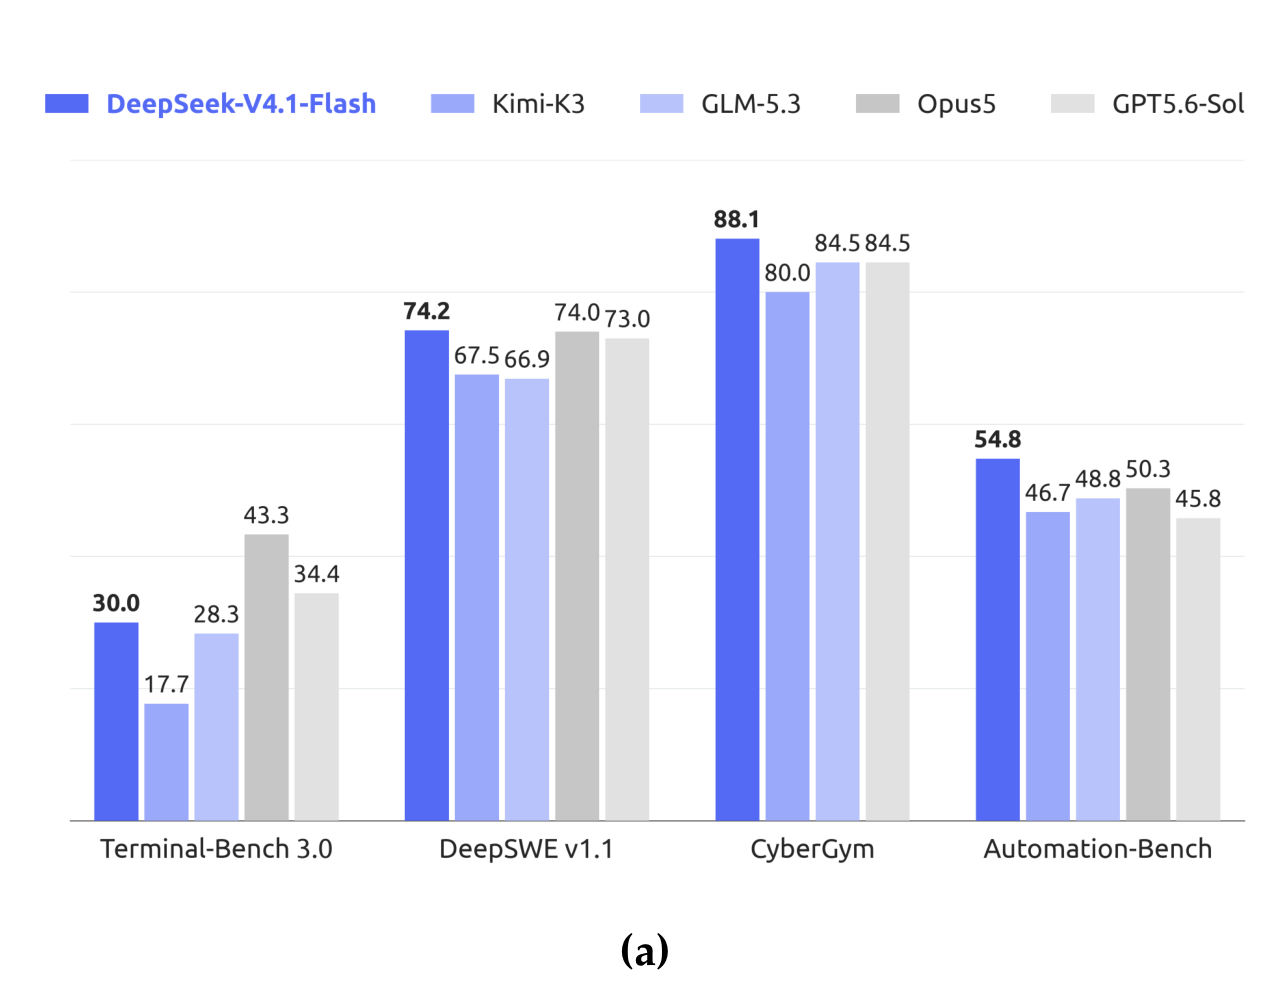
\includegraphics[width=0.48\linewidth]{images_hi/fig01a}
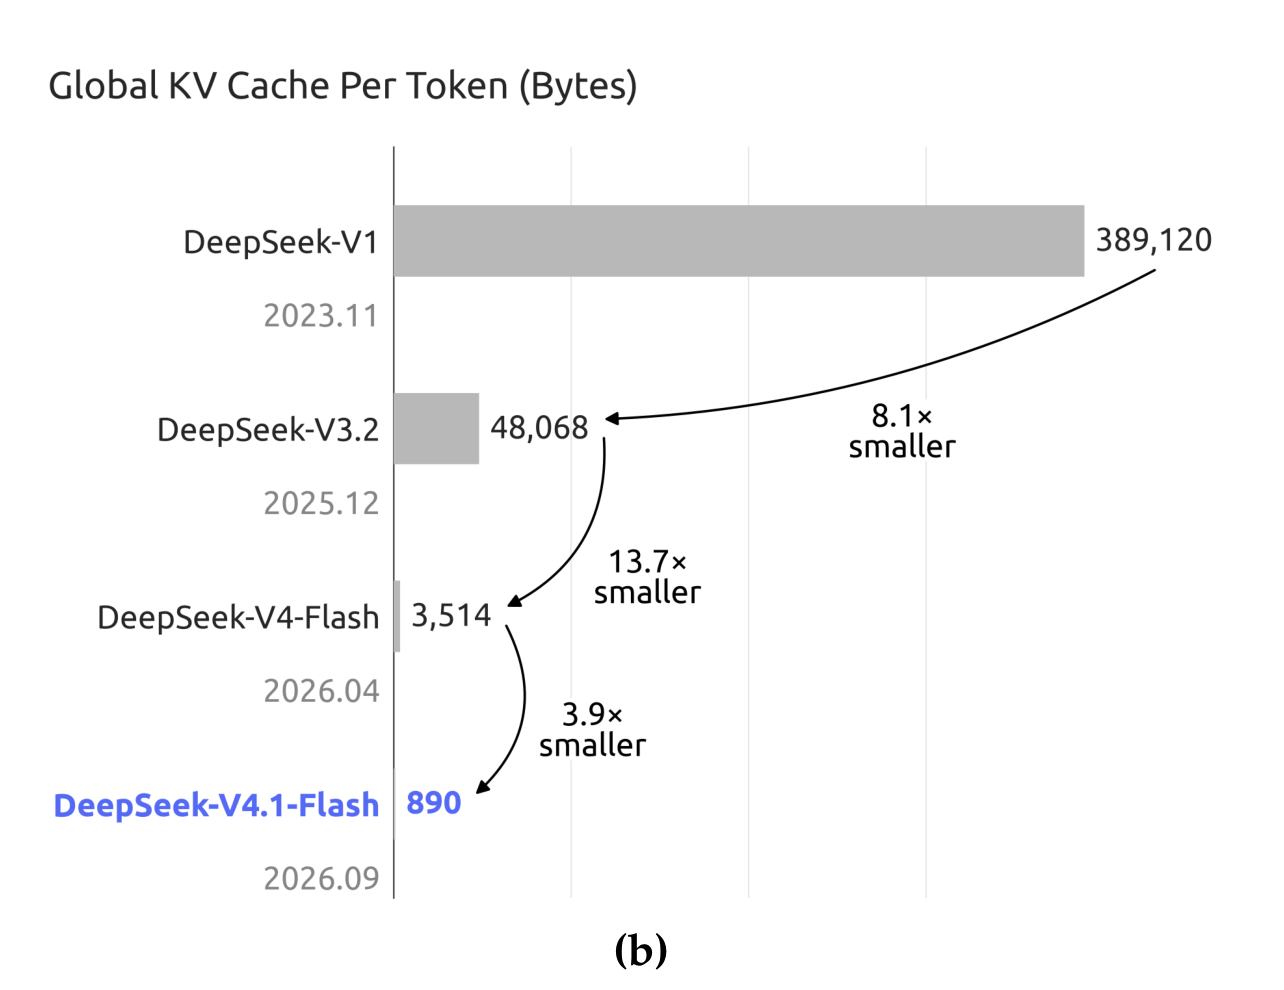
\includegraphics[width=0.48\linewidth]{images_hi/fig01b}
\hfill
\caption{(a) DeepSeek-V4.1-Flash 及其对标模型在智能体基准上的性能。(b) 历代 DeepSeek 模型的每 token 全局 KV 缓存大小（字节），凸显了 DeepSeek 在降低上下文内存需求方面的持续努力。与 DeepSeek-V4-Flash 和 DeepSeek-V1 相比，DeepSeek-V4.1-Flash 的每 token 全局 KV 缓存大小分别实现了约 4 倍与 437 倍的缩减。}
\label{fig:1}
\end{figure}
\begin{figure}[htbp]
\centering
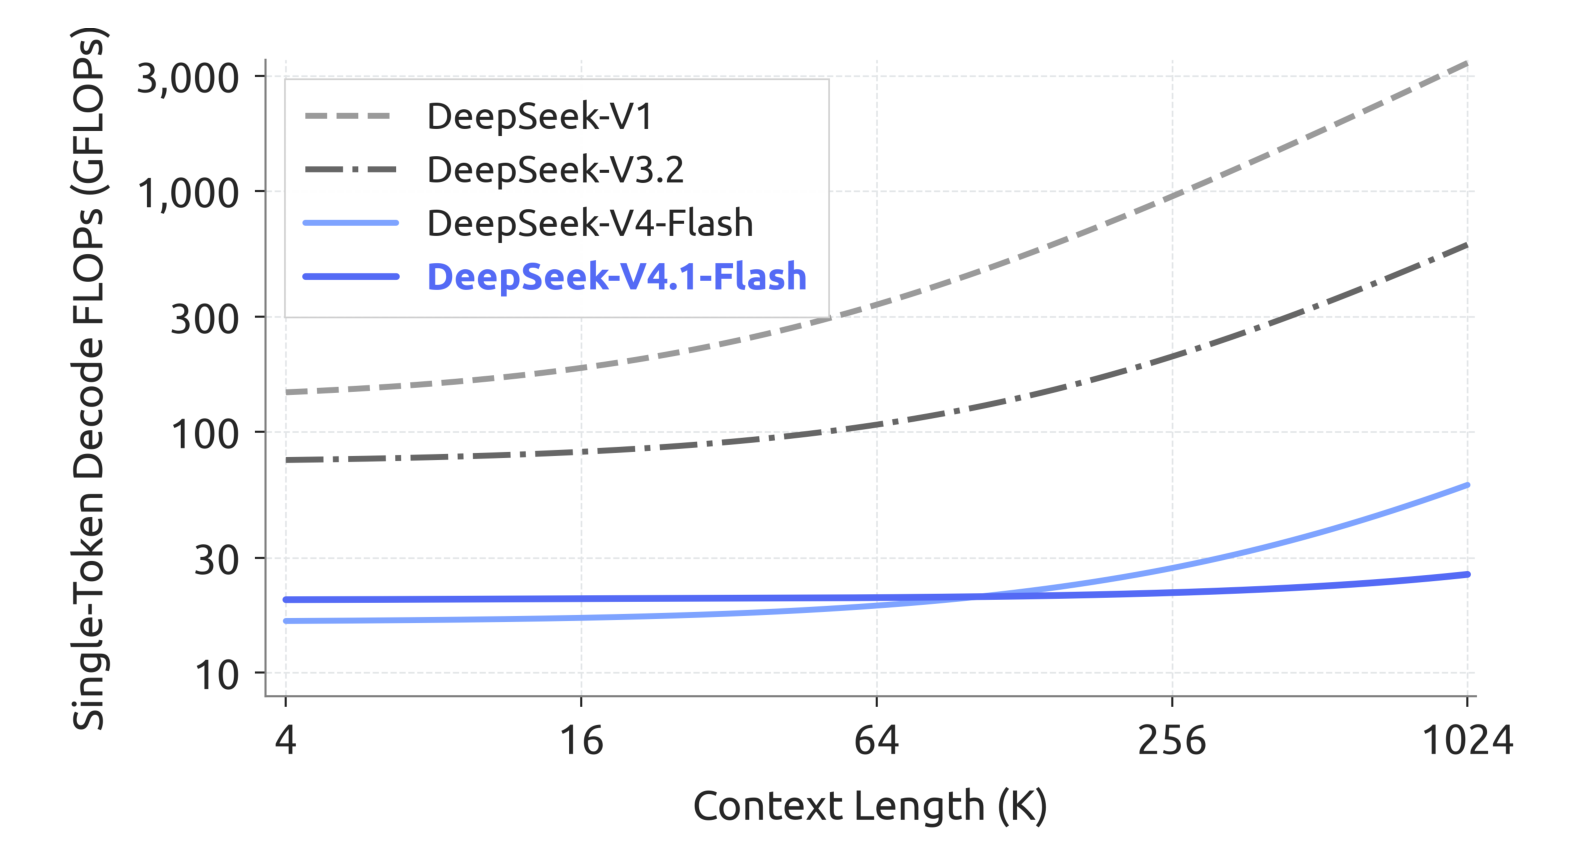
\includegraphics[width=\linewidth]{images_hi/fig02}
\caption{历代 DeepSeek 模型的单 token 解码 FLOPs 随上下文长度的变化。我们按 1、0.5、0.25 分别加权 BF16、FP8 与 FP4 运算，以计入计算精度差异。随着上下文长度增加，DeepSeek-V4.1-Flash 的解码 FLOPs 基本保持恒定，大幅降低了长上下文场景的计算成本。}
\label{fig:2}
\end{figure}
\begin{figure}[htbp]
\centering
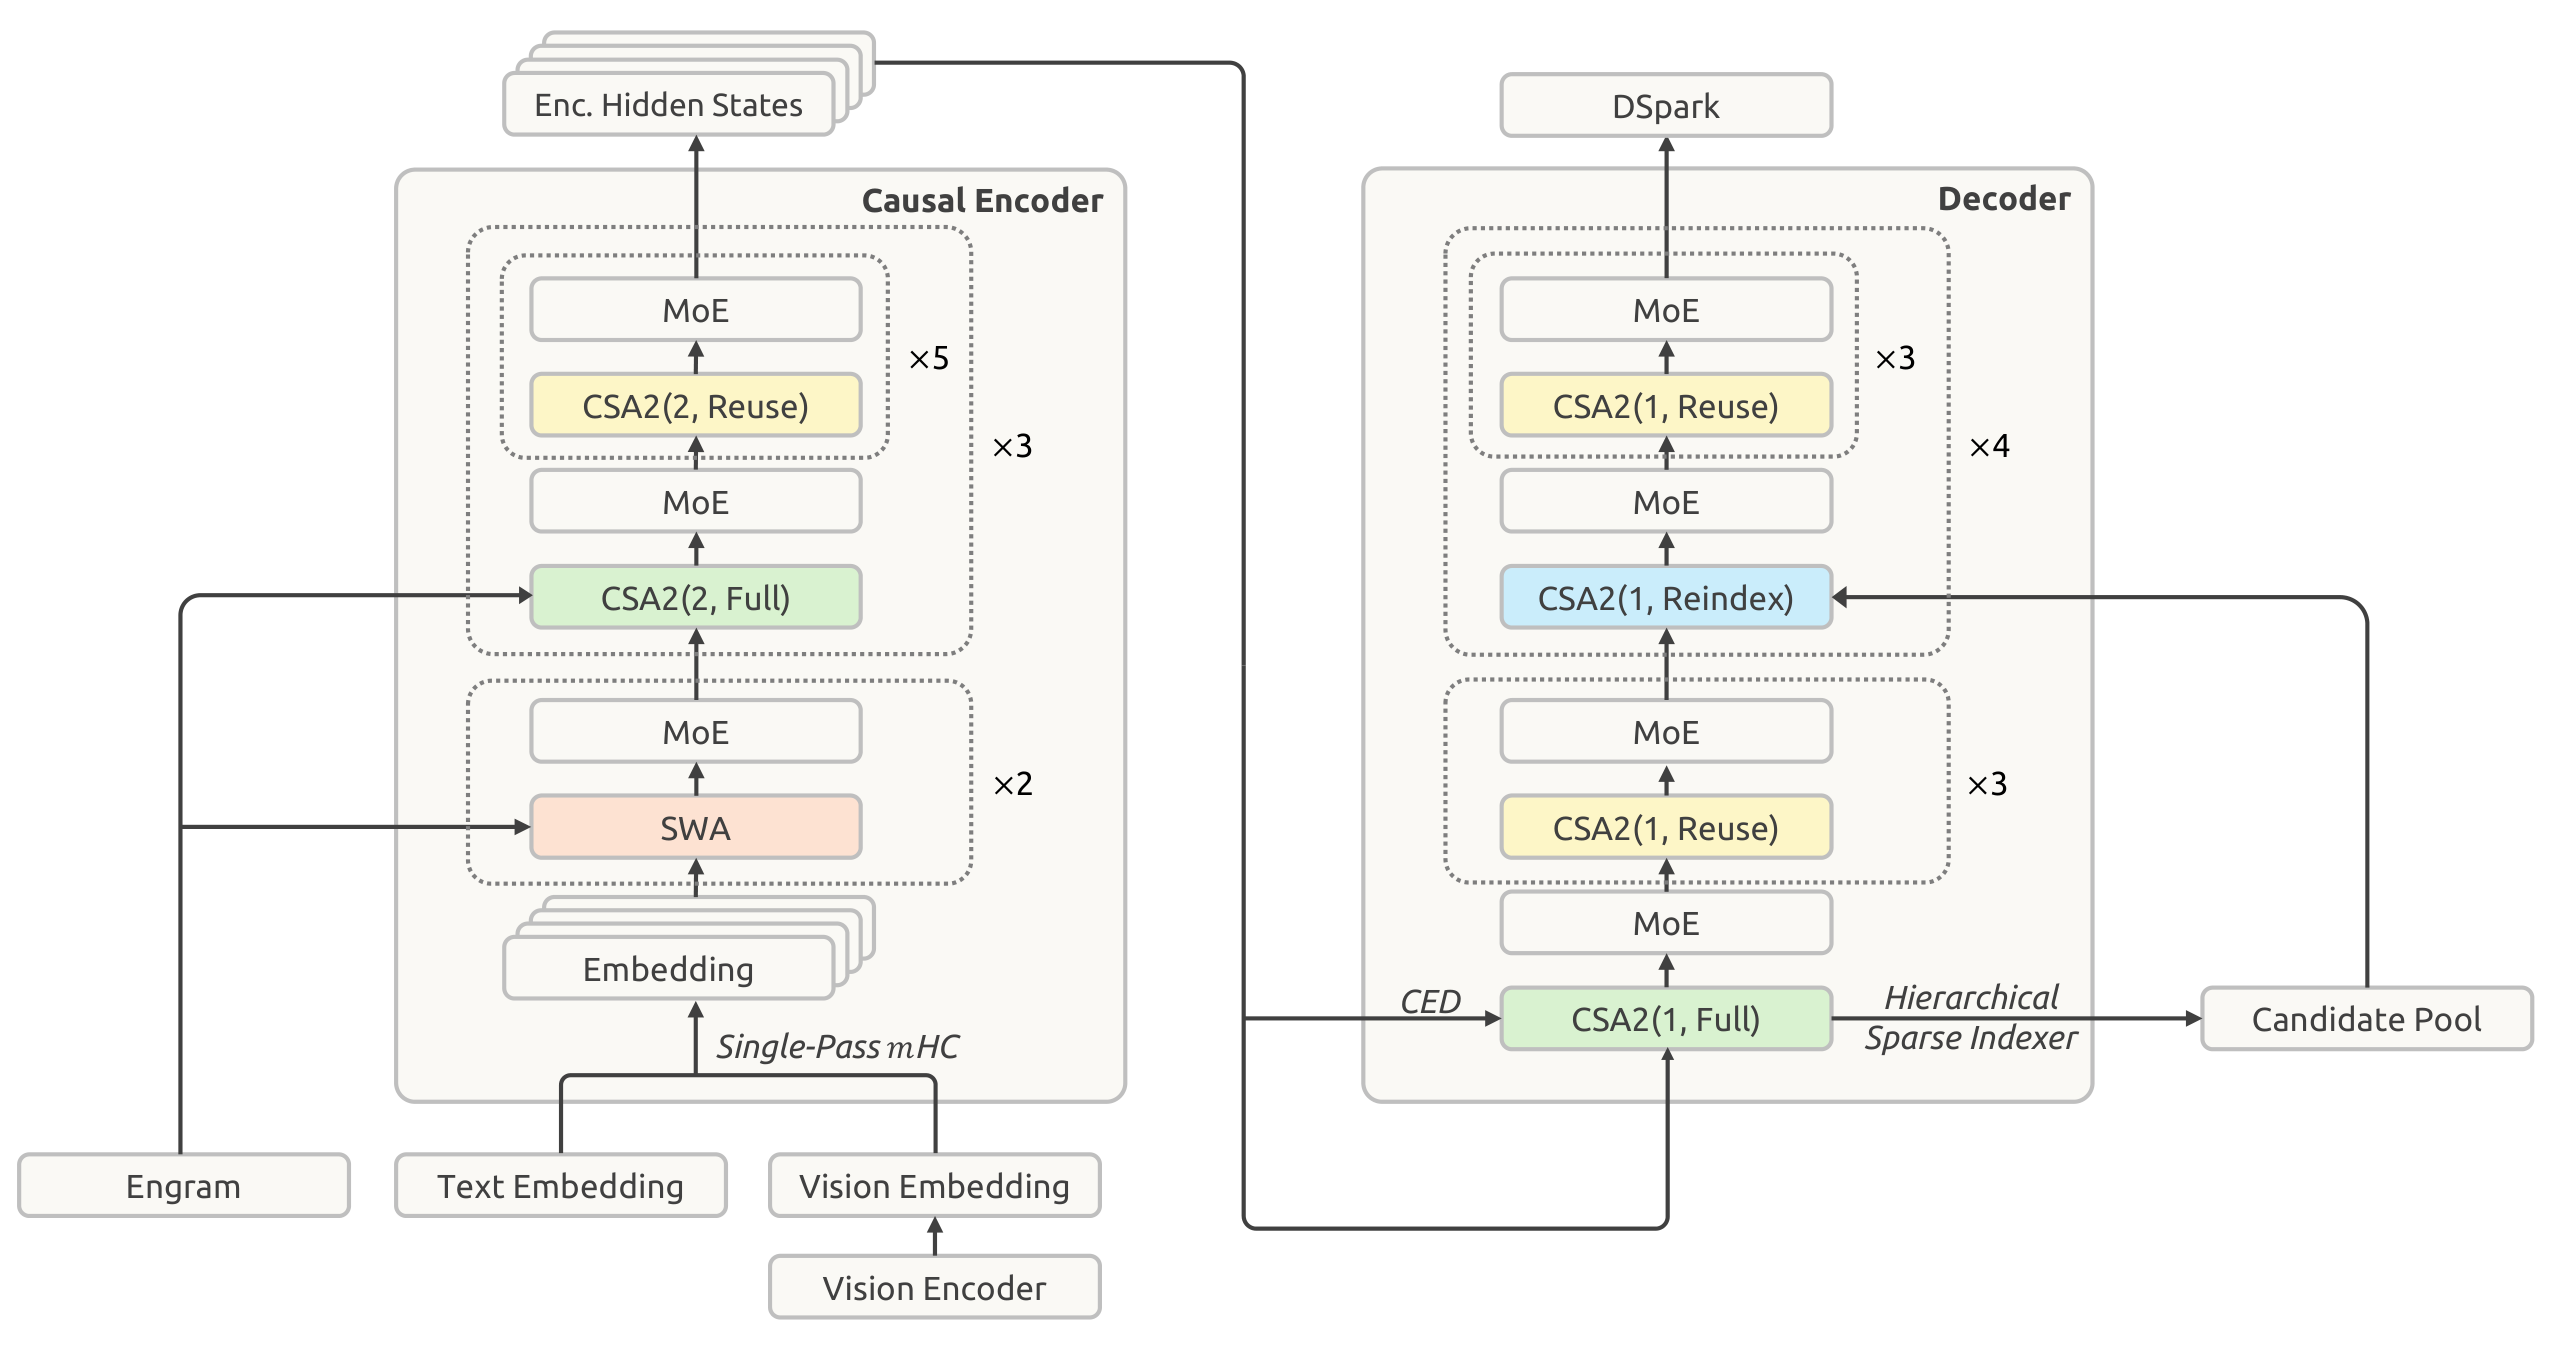
\includegraphics[width=\linewidth]{images_hi/fig03}
\caption{DeepSeek-V4.1-Flash 的整体架构。40 层网络分为因果编码器与解码器两部分，各含 20 层。所有前馈层均使用标准 DeepSeekMoE。前两层编码器使用滑动窗口注意力（SWA），其余层使用压缩稀疏注意力 2（CSA2），其中 CSA2(ratio, mode) 用于指定压缩率与模式。该模型还使用了 Single-Pass mHC、Engram、DSpark 与层级稀疏索引器（Hierarchical Sparse Indexer）。}
\label{fig:3}
\end{figure}